% CoRL 2026 Workshop "Bringing Physics Simulation and World Models Together for Robotic Manipulation" (PhysWM)
% (https://corl26ws-physwm.github.io); accepted as a poster (submission 71). Built from robots_need_wm_camera_ready.
% CAMERA-READY (deadline to be announced). Incorporates the review (aCbS) and the other workshop's two reviews.
%
% Non-archival; 4 pages excluding references (limitations, AI statement and appendix also kept after the body).
% 2026-11-02 rewrite (user): one storyline (fork = safety proxy at the safe-set boundary + test of physical fidelity
% -> benchmark -> why stochastic vs deterministic), intuitive-physics-engine context, why bimodality, Fig. 1 boundary.
% Build: tectonic main.tex (corl_2026.sty, corlabbrvnat.bst: official kit).
\documentclass{article}
\usepackage[preprint]{corl_2026}   % official CoRL 2026 style; [preprint] = de-anonymised without the main-conference footer
\makeatletter\renewcommand{\@noticestring}{CoRL 2026 Workshop on Bringing Physics Simulation and World Models Together for Robotic Manipulation, Austin, TX, USA.}\makeatother
\usepackage[T1]{fontenc}           % Times (ptm) under XeTeX/Tectonic; harmless under pdfLaTeX
\usepackage{booktabs,amsmath,amssymb,graphicx,xcolor,tikz}
\usetikzlibrary{positioning,arrows.meta}
\usepackage{wrapfig}
\definecolor{inkc}{HTML}{1B2430}\definecolor{mutedc}{HTML}{5D6873}\definecolor{linec}{HTML}{C3CAD1}
\definecolor{cardc}{HTML}{F2F4F6}\definecolor{tealc}{HTML}{0E7A86}\definecolor{orangec}{HTML}{C96A14}
\definecolor{violetc}{HTML}{6B55C9}
\newcommand{\todo}[1]{\textcolor{red}{[TODO: #1]}}

\title{Branching Fidelity: Testing World Models as Intuitive Physics Engines for Robot Safety\thanks{A version of this work also appears at the CoRL 2026 Workshop ``Do Robots Need World Models?''.}}
\author{
  Alikasim Budhwani \qquad Soo Jeon\\
  Department of Mechanical and Mechatronics Engineering, University of Waterloo, Canada\\
  \texttt{a2budhwa@uwaterloo.ca}
}

\begin{document}
\maketitle

\begin{abstract}
Near a physical tipping point, the same robot action can succeed or fail depending on a few millimetres of
the robot's own perception and execution error. We call such a state a \emph{fork}: sampled over this
uncertainty, its futures split into separate outcomes. In rigid-body manipulation, where one branch is often
irreversible, a fork marks the boundary between safe and unsafe states without failure labels; and finding
forks needs a simulator that responds to millimetre changes as physics does, so forks also test the
physical fidelity of world models. Our \emph{fork probe} follows the intuitive physics engine of cognitive
science (people judge stability with a few rough mental simulations): it samples the robot's measured
errors, imagines many futures and flags the action if they split. With a physics engine as the upper
reference, it catches 88\% of forks on unseen layouts with 7\% false alarms. A stochastic world model with
3--4$\times$ lower error than predicting that nothing moves catches only 18\%: its noise spreads futures in
every direction, not along the branch. Deterministic dynamics started from perturbed scenes, which put the
uncertainty where it really is, reach 72\%, and 82\% when training oversamples rare branches found by the
probe's own split test. World-model benchmarks should measure this \emph{branching fidelity} beside
average error.
\end{abstract}

\keywords{World models, intuitive physics, uncertainty, safe deployment}

\section{Introduction}
\begin{wrapfigure}{r}{0.43\linewidth}
\vspace{-12pt}
\centering
% Figure 1: a fork is a state whose uncertainty straddles the boundary between safe and unsafe outcomes.
% Schematic (not data). Dots = sampled starts (perception + execution error), coloured by where their future ends.
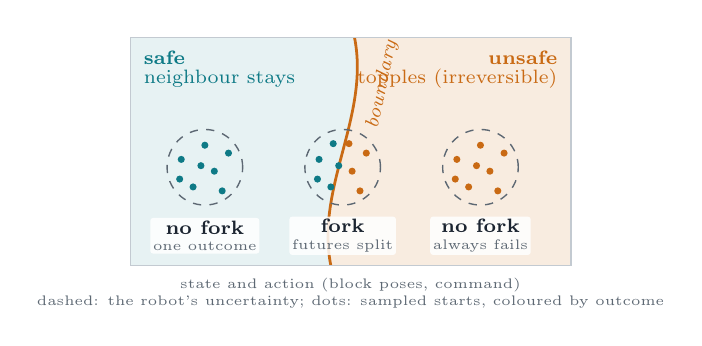
\begin{tikzpicture}[font=\scriptsize, x=1cm, y=1cm]
\def\bnd{(2.55,0) .. controls (2.35,1.0) and (3.05,1.9) .. (2.85,2.9)}
\fill[tealc!10] (0,0) -- \bnd -- (0,2.9) -- cycle;
\fill[orangec!13] (5.6,0) -- (2.55,0) .. controls (2.35,1.0) and (3.05,1.9) .. (2.85,2.9) -- (5.6,2.9) -- cycle;
\draw[orangec, line width=1pt] \bnd;
\draw[linec, line width=0.4pt] (0,0) rectangle (5.6,2.9);
\node[anchor=north west, text=tealc, font=\scriptsize\bfseries, align=left] at (0.05,2.85) {safe\\[-1pt]\mdseries neighbour stays};
\node[anchor=north east, text=orangec, font=\scriptsize\bfseries, align=right] at (5.55,2.85) {unsafe\\[-1pt]\mdseries topples (irreversible)};
\node[text=orangec, font=\scriptsize\itshape, rotate=78] at (3.2,2.3) {boundary};
% the robot's uncertainty around three nominal states
\foreach \cx/\cy/\lab/\sub in {0.95/1.25/no fork/one outcome, 2.7/1.25/fork/futures split, 4.45/1.25/no fork/always fails} {
  \draw[mutedc, dashed, line width=0.5pt] (\cx,\cy) circle (0.48);
  \node[font=\scriptsize\bfseries, text=inkc, fill=white, fill opacity=0.85, text opacity=1, inner sep=1pt, rounded corners=1pt, align=center] at (\cx,0.38) {\lab\\[-2pt]\mdseries\tiny\textcolor{mutedc}{\sub}};
}
\foreach \dx/\dy in {-0.3/0.1, -0.15/-0.25, 0/0.28, 0.12/-0.05, 0.3/0.18, -0.05/0.02, 0.22/-0.3, -0.32/-0.15}
  \fill[tealc] (0.95+\dx,1.25+\dy) circle (0.045);
\foreach \dx/\dy in {-0.3/0.1, -0.15/-0.25, 0/0.28, 0.12/-0.05, 0.3/0.18, -0.05/0.02, 0.22/-0.3, -0.32/-0.15}
  \fill[orangec] (4.45+\dx,1.25+\dy) circle (0.045);
\foreach \dx/\dy/\c in {-0.3/0.1/tealc, -0.15/-0.25/tealc, -0.05/0.02/tealc, -0.32/-0.15/tealc, -0.12/0.3/tealc,
                        0.12/-0.05/orangec, 0.3/0.18/orangec, 0.22/-0.3/orangec, 0.08/0.3/orangec}
  \fill[\c] (2.7+\dx,1.25+\dy) circle (0.045);
\node[anchor=north, font=\tiny, text=mutedc, align=center] at (2.8,-0.04)
  {state and action (block poses, command)\\dashed: the robot's uncertainty; dots: sampled starts, coloured by outcome};
\end{tikzpicture}

\vspace{-14pt}
\caption{A fork is a state whose uncertainty straddles the boundary between safe and unsafe outcomes.}
\label{fig:boundary}
\vspace{-10pt}
\end{wrapfigure}
Manipulation policies act by committing to short action chunks
\citep{chi2023diffusion,zhao2023act,black2024pi0}. Before each chunk runs, a safe robot should ask: could
my own small errors change what happens? When a robot picks a block standing between two others, the same
command can lift it cleanly or tip a neighbour, depending on a few millimetres of perception and execution
error. Existing monitors flag inputs a model has not seen \citep{seo2025uncertainty,xu2025failure}; this
\emph{physical} uncertainty remains even for a perfect model.

Cognitive science describes how people handle this. In the \emph{intuitive physics engine} account
\citep{battaglia2013simulation,smith2013sources,sanborn2013reconciling}, people judge whether a stack will
fall by simulating it in their heads a few times, each with slightly different guesses of where things
are, and call it precarious when the outcomes disagree. We give robots the same check, with measured
errors in place of guesses, and call a state whose imagined futures split a \emph{fork}
(Fig.~\ref{fig:boundary}).

Forks connect two questions. \textbf{Safety:} in rigid-body manipulation one branch is often
irreversible: a toppled block stays toppled. A fork then marks a state one small error away from the
unsafe set, i.e.\ the boundary of the safe set, found without failure labels. It is a proxy, not a failure
detector: both branches may be harmless, and an action that always fails lies inside the unsafe set and
never splits. \textbf{Physical fidelity:} to find forks, the simulator must respond to millimetre changes
of state and action as physics does; its futures must branch where physics branches. Outside simulation
that simulator is a learned world model, and its average prediction error, dominated by states where
nothing dramatic happens, does not test this sensitivity. We call it \emph{branching fidelity} and measure
it by fork detection.

\paragraph{Contributions.} (1) A label-free \emph{fork probe} (Sec.~\ref{sec:probe}). (2) With a physics
engine, the probe catches 88\% of forks from one camera image: the level a world model should reach
(Sec.~\ref{sec:validation}). (3) A branching-fidelity benchmark of world models: why stochastic models
fail despite good average accuracy, why deterministic ones with uncertain starts come close, and how the
split test improves training (Sec.~\ref{sec:wm}).

\section{The fork probe}\label{sec:probe}
\paragraph{Task.} A simulated Franka Panda (MuJoCo) must pick the middle of three upright blocks without
toppling its neighbours (Fig.~\ref{fig:forks}a). A policy commits to 8-step action chunks; the probe
treats it as a black box and sees only the chunk, one camera image and the robot's joint state.

\begin{figure}[t]
\centering
% Figure 1 (a): the fork probe as a pipeline. Images: exact replays of held-out state ep63_seed104_s74
% (paper/render_fork_frames.py). Ghost images average the 64 imagined starts / endings.
\begin{tikzpicture}[
  font=\footnotesize, every node/.append style={execute at begin node={\hyphenpenalty=10000\relax}},
  stage/.style={font=\scriptsize\bfseries\color{inkc}, anchor=south},
  note/.style={font=\scriptsize, text=mutedc, align=center, anchor=north, text width=2.3cm},
  img/.style={inner sep=0pt, draw=linec, line width=0.4pt},
  card/.style={draw=linec, fill=cardc, rounded corners=3pt, line width=0.4pt, align=center,
               minimum height=2.15cm, inner sep=3pt, font=\scriptsize},
  flow/.style={-{Stealth[length=4pt]}, line width=0.7pt, draw=mutedc},
]
\def\w{2.15cm}
% 1 camera image
\node[img] (cam) at (0,0) {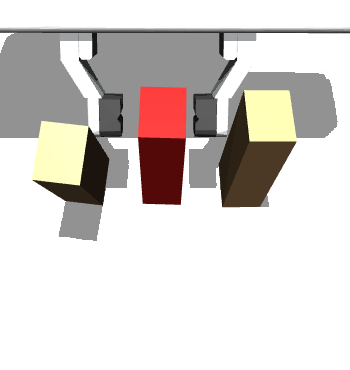
\includegraphics[width=\w]{fig_assets/crop_start.png}};
\node[stage] at (cam.north) {camera image};
\node[font=\small\bfseries, anchor=south east] at ([xshift=-2pt,yshift=10pt]cam.north west) {(a)};
\node[note] at (cam.south) {perceived block poses\\(2.5\,mm error)};
% 2 the robot's uncertainty
\node[img, right=0.55cm of cam] (unc) {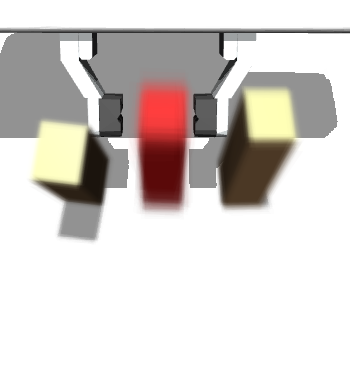
\includegraphics[width=\w]{fig_assets/crop_start_ghost.png}};
\node[stage] at (unc.north) {\textcolor{tealc}{its own uncertainty}};
\node[note] at (unc.south) {$N$ plausible scenes (measured perception error) $\times$ measured execution error};
% 3 rollout engine
\node[card, right=0.55cm of unc, text width=2.15cm] (eng) {%
  \textbf{rollout engine}\\[3pt]
  8-step chunk\\then 30-step\\imagined hold\\[4pt]
  \textcolor{inkc}{MuJoCo}\\{\color{mutedc}(reference)}\\[1pt] or\\[1pt]
  \textcolor{violetc}{learned world model}};
% 4 imagined futures
\node[img, right=0.55cm of eng] (fut) {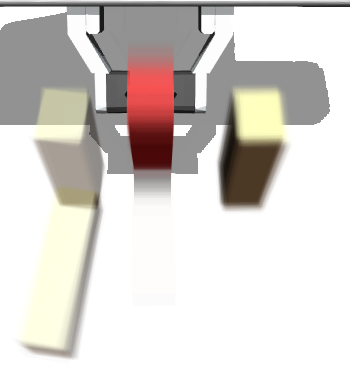
\includegraphics[width=\w]{fig_assets/crop_end_ghost.png}};
\node[stage] at (fut.north) {\textcolor{orangec}{$N$ imagined futures}};
\node[note] at (fut.south) {the neighbour stays (31)\\or topples (33)};
% 5 decision
\node[card, right=0.55cm of fut, text width=1.9cm] (dec) {%
  \textbf{split test}\\[3pt]
  two persistent,\\well-separated\\groups?\\[4pt]
  \textcolor{orangec}{\textbf{yes: fragile}}\\[1pt]
  {\color{mutedc}slow down,\\re-perceive, replan}};
\draw[flow] (cam.east) -- (unc.west);
\draw[flow] (unc.east) -- (eng.west);
\draw[flow] (eng.east) -- (fut.west);
\draw[flow] (fut.east) -- (dec.west);
\end{tikzpicture}
\\[1pt]
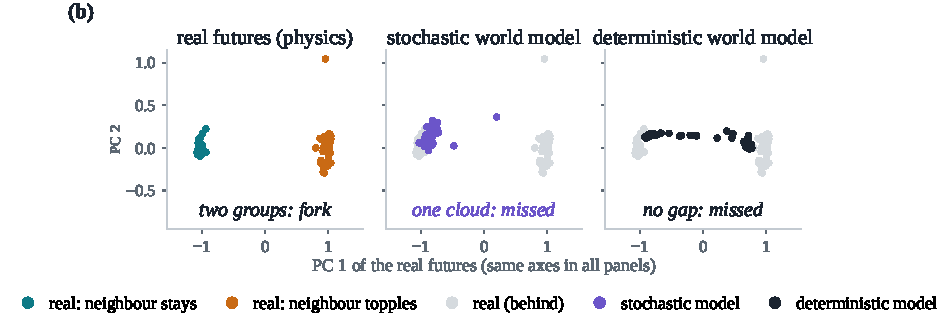
\includegraphics[width=0.93\linewidth]{fig_futures.pdf}
\caption{(a) The fork probe on one held-out state ($N=64$; exact renders, images average all samples).
(b) The $N$ futures of that state, projected on the real futures' two main axes. The real futures form
two groups (the neighbour stays or topples). The stochastic world model's futures form one cloud, so no
fork is detected; the deterministic model's futures stretch along the branch but leave no gap.}
\label{fig:forks}
\end{figure}

\paragraph{Forks.} The simulated physics is deterministic, so all uncertainty is the robot's own: its
error in perceiving the block poses (2.5\,mm, measured on held-out images) and in executing commands
(about 3\,mm, measured from tracking). A state is a fork if the outcome splits over $N=64$ futures sampled
from this uncertainty: here, if between 2 and 62 of them topple a neighbour.

\paragraph{Probe.} The probe imagines $N$ versions of the chunk. Each starts from the perceived scene
shifted by a sampled perception error and runs the chunk with a sampled execution error; the robot then
holds still for 30 steps so the outcome settles. The probe flags the chunk if the $N$ endings fall into
two separate groups. We test for separate groups (bimodality), not for large spread: futures can differ
smoothly without a change of outcome (a block sliding a few millimetres further), whereas a fork is a
qualitative split with a gap, and a spread threshold would need tuning per task. The split test uses
fixed statistical conventions, not thresholds fit to labels (Appendix~\ref{app:details}).
The simulator can be swapped. Our reference is MuJoCo given the blocks' true shapes, masses and
friction, which a real robot does not know: not a deployable baseline but the \emph{upper reference}, the
branching a learned world model should reproduce (Sec.~\ref{sec:wm}).

\paragraph{Ground truth.} One real outcome cannot grade the probe, since a fragile action may succeed by
luck. An oracle runs the $N$ futures from the \emph{true} scene in exact physics and labels forks as above;
two independent oracle runs agree on 99\% of states. Each test set has unseen block layouts, about 60
forks and 100 safe states, and was fixed before testing.

\section{Results}
\subsection{With a physics engine, the probe works}\label{sec:validation}
Sampling the perception error matters: a probe that trusts the pose estimate catches only 65--67\% of
forks, because perception errors are as large as execution errors; sampling them raises this to
77--91\% (Table~\ref{tab:panels}). Reading the endings from image features instead of block positions
changes little: on test set C the probe catches 88\% of forks (95\% CI 77--94\%) with 7\% false alarms.
This is the bar a learned world model must reach.

\begin{table}[t]
\centering
\caption{The fork probe with a physics engine on three unseen test sets: forks caught / false alarms (\%).}
\label{tab:panels}
\small
\begin{tabular}{lcccccc}
\toprule
& \multicolumn{2}{c}{Set A (153 states)} & \multicolumn{2}{c}{Set B (160)} & \multicolumn{2}{c}{Set C (156)} \\
& caught & false & caught & false & caught & false \\
\midrule
pose estimate trusted (no perception sampling) & 65 & 23 & 65 & 12 & 67 & 24 \\
fork probe, endings read from block positions & 90 & 12 & 77 & 8 & 91 & 10 \\
fork probe, endings read from images & 88 & 12 & 77 & 8 & \textbf{88} & \textbf{7}$^*$ \\
\bottomrule
\multicolumn{7}{l}{\footnotesize $^*$ with 5 sampled scene estimates (Appendix~\ref{app:details}); 9\% with one.}
\end{tabular}
\end{table}

\subsection{Benchmarking world models by branching fidelity}\label{sec:wm}
A learned model now takes MuJoCo's role. Our models predict in a compact DINOv2 feature space
\citep{oquab2024dinov2} (Appendix~\ref{app:details}); each training image comes with 8 real futures from
perturbed starts, so a model can learn the robot's own uncertainty. We compare a stochastic
model (flow matching), which draws fresh noise at every step, with a deterministic one that predicts the
next state directly. Both have 3--4$\times$ lower prediction error than simply predicting that nothing
moves, yet on test set C the stochastic model catches 18\% of forks and the deterministic one 60\%
(Table~\ref{tab:wm}).

\begin{table}[t]
\centering
\caption{World models. Spread: total spread of the futures relative to real futures; main axis: its
share along the real futures' main axis; fork ratio: spread on forks over spread on safe states. Fresh
test sets were never used for training or selection.}
\label{tab:wm}
\small
\begin{tabular}{lccccc}
\toprule
rollouts from & caught & false & spread & main axis & fork ratio \\
\midrule
\multicolumn{6}{l}{\emph{test set C (156 states)}} \\
physics engine (upper reference) & 88\% & 7\% & 1.00 & 0.57 & 4.8 \\
world model, stochastic & 18\% & 2\% & 0.98 & 0.15 & 1.3 \\
world model, deterministic & 60\% & 10\% & 0.04 & 0.69 & 32 \\
\midrule
\multicolumn{6}{l}{\emph{two fresh test sets (160 / 152 states)}} \\
uncertain starts + deterministic & 72 / 82\% & 8 / 7\% & & & \\
\quad + rare-branch oversampling & 82 / 85\% & 9 / 11\% & & & \\
\bottomrule
\end{tabular}
\end{table}

\paragraph{Why the stochastic model fails.} In physics, futures differ only because starts and commands
differ, and they diverge only near the boundary. The stochastic model instead adds noise at every step.
It learns the right \emph{amount} of spread (0.98 of the real futures') but not \emph{where} it belongs:
its futures spread in every direction, almost as much on safe states as on forks (fork ratio 1.3 vs 4.8
for physics; Fig.~\ref{fig:forks}b). Five further generative variants catch at most 3\% of forks, with
the same shapeless spread (Appendix~\ref{app:details}).

\paragraph{Why the deterministic model comes closer.} Its futures differ only through their perturbed
inputs, so, as in physics, its spread comes from the sensitivity of its dynamics: tiny overall, but along
the branch and 32$\times$ larger on forks. Its weakness is the opposite one: trained with squared error,
it predicts the average of the outcomes it has seen, so near a fork its futures stretch toward both
branches without a gap (Fig.~\ref{fig:forks}b), and rare branches get averaged away.

\paragraph{Uncertain starts.} As in the intuitive physics engine, uncertainty should enter where it really
is: in the robot's knowledge of the scene, not in the physics. A learned operator perturbs the start by
sampled perception error and the deterministic model rolls each start out. Trained on fork-rich data, this
catches 72\% of forks on a fresh test set and plateaus there: longer training, more data, a frame history
or DINO-WM's transformer predictor \citep{zhou2025dinowm} all land at 68--72\%. A generative model given
the same perturbed starts still catches 0\%: the noise in its dynamics erases the forks.

\paragraph{The split test also improves training.} Without labels, we apply the split test to each
training scene's own real futures, mark the smaller group as the rare branch, and fill half of every batch
with rare-branch futures. On two fresh test sets this lifts the uncertain-start model from 72 to 82\% and
from 82 to 85\% of forks: branching fidelity can be trained for, not only measured.

\section{Related work}
Robotics runs Monte Carlo rollouts over pose, friction or model parameters to score grasps and pushes
\citep{mahler2017dexnet,agboh2018pushing}, build safety filters \citep{johansson2025safety,wang2026manidreams}
or judge whether blocks stay standing \citep{cannizzaro2024cobra,zhou2023mental,lerer2016learning};
\citet{goyal2026stability} and \citet{zapolsky2016particle} measure how perturbed rollouts diverge. These
predict a task outcome, a stability label or a divergence rate; our probe is a per-chunk Monte Carlo test
of closeness to a basin boundary \citep{menck2013basin}. Safety filters and failure detectors use failure
labels, epistemic or policy uncertainty \citep{nakamura2025generalizing,seo2025uncertainty,xu2025failure,agia2024unpacking}:
what a model does not know, not whether the physics is at a branch. Learned world models
\citep{sanchezgonzalez2020learning,allen2023fignet,zhou2025dinowm,assran2025vjepa2,hafner2025dreamerv3}
struggle with stiff contact \citep{parmar2021fundamental} and physical grounding
\citep{bear2021physion,motamed2026physicsiq,yang2026mirabench}; \citet{yu2026evaluated} evaluate branches
created by different actions, ours arise from one action under small errors. Stochastic and ensemble models
\citep{chua2018pets,lakshminarayanan2017ensembles} are judged by likelihood, calibration or return, none of
which checks where their spread splits.

\section{Conclusion}\label{sec:conclusion}
Forks link robot safety and the physical fidelity of world models: in rigid-body manipulation a fork
marks the boundary of the safe set without labels, and finding it needs a simulator that responds to small
changes as physics does. World models with good average accuracy can still miss the branch; the closest
recipe is deterministic dynamics with the uncertainty in the start and rare branches oversampled.
Benchmarks should report branching fidelity beside average error. A fork is not a failure, so a robot
should pair the flag with a harm signal such as whether the outcome can be undone; our follow-up work
builds a label-free safety filter on this recipe. Next: pretrained world models such as V-JEPA 2-AC,
other tasks, and a real robot.

\section*{Limitations}
\begin{itemize}\setlength{\itemsep}{1pt}\setlength{\parskip}{0pt}
\item \textbf{Scope.} Simulation only, one task with three blocks; other tasks, real images and real
robots are untested, and there is no closed-loop intervention or latency experiment here.
\item \textbf{Forks as a safety proxy.} A fork signals danger only when one branch is harmful, as for
toppling rigid bodies. Forks with two harmless branches are false alarms for safety, actions that always
fail are never forks, and gradual harm (deformation, spills) need not split into separate groups.
\item \textbf{Ground truth.} The fork label uses the same perception and execution error model that the
probe samples, so it measures agreement with that model, not with real outcomes; a real-robot anchor is
needed. One Gaussian models perception error for all images, and the engine probe uses the simulator's
true shapes, masses and friction. Sampled pose errors were applied without letting the blocks settle; a
later check found that this moves a block with the robot still in 3 of 25 three-block states.
\item \textbf{Split test.} It projects the endings on one main axis and fits at most two Gaussians, so it
cannot represent more than two outcome regimes and can miss a split along a minor axis.
\item \textbf{Operating points.} Each method is reported at one operating point fixed before testing; a
sweep is possible only for the physics-engine probes on set C (Appendix~\ref{app:sweep}). The test sets
differ in difficulty.
\item \textbf{World models.} Each was trained once, at small scale, from scratch; the DINO-WM comparison
re-implements its predictor on our latents rather than using the released model. The fork-rich training
data of the uncertain-start models was screened with topple counts; only the rare-branch oversampling is
label-free, and the oversampled model also used a faster training recipe.
\end{itemize}

\paragraph{AI usage statement.} Generative AI tools (Claude) assisted with code, figures, literature
search and drafting. The authors designed the study, checked all results and references, and take full
responsibility for the content.

\bibliography{references}

\appendix
\section{Implementation details}\label{app:details}
\paragraph{Uncertainty model.} Execution error is drawn from 64 snippets of the robot's measured tracking
residuals (median per-chunk maximum 3.2\,mm). Perception is a frozen DINOv2 encoder on one close-camera
image with a small head that predicts the three blocks' poses (2.5\,mm held-out error); its error model
is a zero-mean Gaussian fitted once, offline, to its errors on held-out images with known poses (a full
$9\times9$ position covariance capturing correlated errors, plus rotation covariances).

\paragraph{Actions and the hold.} An action is an absolute end-effector position target plus a gripper
command, tracked by an impedance controller for 0.1\,s. Chunk step $k$ executes the commanded target plus
the sampled execution error; during the 3\,s hold the arm holds the chunk's last nominal target, without
execution error. The world models receive exactly the same action sequence, with no special hold input.

\paragraph{Split test.} The 64 endings (block positions, or DINOv2 features of the rendered endings) are
projected on their first principal axis at hold steps 10 and 30. The chunk is flagged if, at both times,
two Gaussians fit better than one (BIC), the groups are well separated (Ashman's $D>2$
\citep{ashman1994detecting}) and the smaller group has at least 2 members, and the grouping is the same
at both times. These are fixed statistical conventions, not fitted to labels.

\paragraph{Five scene hypotheses.} Each hypothesis draws one scene estimate from the perception-error model
around the perceived scene; its 64 futures add a fresh perception draw and an execution-error sample
each. The probe flags if at least 3 of the 5 hypotheses split.

\paragraph{Ground truth.} The oracle is the probe centred on the true scene: each of its 64 futures starts
from the true block poses shifted by a fresh perception-error draw and uses one execution-error sample (the
same 64 snippets as the probe, different perception seeds). A neighbour topples if it tilts more than
45$^\circ$ by the end. Test-set states were found by an execution-only screen, not by the oracle.

\paragraph{World models.} The latent compresses DINOv2 patch tokens by a fixed per-patch PCA to
$28\times28\times8$; applied to real futures, the split test on this latent still catches 97\% of forks.
The dynamics are a convolutional network with six residual blocks conditioned on the action. One model
step covers two simulator actions (0.2\,s), so the 8-step chunk plus the 30-step hold is 19 model steps;
the quoted prediction error is the open-loop latent error at the end of this horizon (0.055 stochastic,
0.042 deterministic, 0.176 for predicting that nothing moves, i.e.\ copying the current latent). The stochastic model is a flow-matching transition
that draws fresh noise at every step; the deterministic one predicts the next latent directly. Each
training image comes with 8 real futures whose starts were perturbed by sampled perception error.

\paragraph{Generative variants.} Whole-clip generation, an energy-score loss, 4$\times$ more fork data,
and an action-sensitivity loss. On 160 held-out states from the training domain (75 forks) they catch
0--3\% of forks at 0--1\% false alarms, with spread 1.1--1.6$\times$ that of the real futures and only
7--10\% of it on the main axis.

\paragraph{Uncertain starts.} A learned operator perturbs the start latent by a sampled perception error
and the deterministic network rolls each perturbed start out. On the 160 training-domain states it
catches 52\% of forks at 7\% false alarms, and 69\% at 8\% with 4$\times$ more fork-rich data; there,
the perturbations were paired with the real futures' own draws. On the fresh test sets every draw is
independent, as in deployment. Variants with 3$\times$ longer training, more fork data, a 3-frame history
or DINO-WM's transformer predictor \citep{zhou2025dinowm} reach 68--72\% on the training-domain states.

\paragraph{Rare-branch oversampling.} For every training state, the split test is applied to the latents
of its real futures; if it splits, the smaller group at hold step 30 is the rare branch. Each batch draws
half its futures from rare branches and half from the other branch of the same starts. Model and loss are
unchanged, but this model was trained with a faster recipe (larger batches, the same number of samples);
a model without oversampling was not retrained with that recipe. The fresh test sets have 160 states
(67 forks) and 152 states (55 forks), with reset seeds disjoint from training but chunks from the same 100
demonstrations; neither was used for training or model selection. The first had earlier served as a
held-out check for other models; the second was generated for this check.

\section{Operating-point sweep}\label{app:sweep}
\begin{figure}[h]
\centering
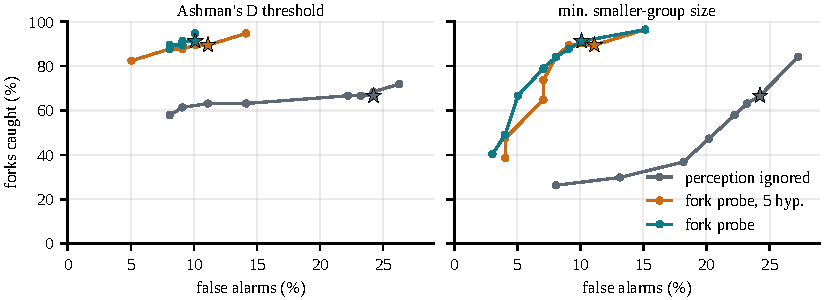
\includegraphics[width=\linewidth]{fig_sweep.pdf}
\caption{Forks caught vs false alarms on test set C (57 forks, 99 safe states) as one split-test setting
is varied with the others at their defaults; stars mark the defaults used in Table~\ref{tab:panels}.
Left: Ashman's $D$ threshold (0.5--8). Right: minimum size of the smaller group (1--16).}
\label{fig:sweep}
\end{figure}
Recomputed from the stored set-C rollouts, the defaults reproduce Table~\ref{tab:panels} exactly. Across
every Ashman's-$D$ threshold from 0.5 to 8, the fork probe catches 88--95\% of forks at 8--10\% false
alarms, while the probe that ignores perception uncertainty never catches more than 72\%, and only 58\%
once its false alarms fall to 8\%. Results barely move between $D=1.5$ and 4, so the default is not a
tuned optimum. The minimum group size is the most sensitive setting: requiring at least 8 members per
group halves every method's catch rate. With five scene hypotheses, requiring 2, 3 or 4 of the 5 to split
gives 95/21, 89/11 and 84/7\% (caught / false); adding a margin to the BIC comparison changes little up
to +10. The probes' advantage holds at every operating point. Rollouts for sets A and B and for the
world models were not stored, so this sweep covers the physics-engine probes on set C only.

\end{document}
